\documentclass[12pt]{extarticle}
\usepackage{tempora}
\usepackage[T1, T2A]{fontenc}
\usepackage[utf8]{inputenc}
\usepackage[english, ukrainian]{babel}
\usepackage{geometry}
\usepackage{graphicx}
\usepackage{multirow}
\usepackage{multicol}
\usepackage{float}
\graphicspath{{/home/artem/Pictures}}
\geometry
{
    a4paper,
    left=30mm,
    top=15mm,
    right=20mm,
    bottom=15mm,
}

\begin{document}
\begin{titlepage}
    \begin{center}
        \textbf{\normalsize{\MakeUppercase{
            Міністерство Освіти і науки України
            Національний університет "Львівська політехніка"
        }}}

        \begin{flushright}
        \textbf{ІКНІ}\\
        Кафедра \textbf{ПЗ}
        \end{flushright}
        \vspace{15mm}

        \includegraphics[width=0.4\textwidth]{lpnu_logo.png}

        \vspace*{\fill}

        \textbf{\normalsize{\MakeUppercase{Звіт}}}
            
        До лабораторної роботи №4

        \textbf{на тему:} “Складення та відлагодження циклічної програми мовою асемблера
        мікропроцесорів х86 для Windows”

        \textbf{з дисципліни:} “Архітектура комп’ютера”
            
        \vspace*{\fill}

        \begin{flushright}

            \textbf{Лектор:}\\
            доцент кафедри ПЗ\\
            Крук О.Г.\\
            \vspace{12pt}

            \textbf{Виконав:}\\
            студент групи ПЗ-24\\
            Губик А. С.\\
            \vspace{12pt}

            \textbf{Прийняв:}\\
            доцент кафедри ПЗ\\
            Задорожний І. М.\\
        \vspace{12pt}
        \end{flushright}

        Львів -- 2023
            
            
    \end{center}
\end{titlepage}

\textbf{Тема роботи:} Складення та відлагодження циклічної програми мовою асемблера
        мікропроцесорів х86 для Windows.

\vspace{12pt}

\textbf{Мета роботи:} ознайомитись на прикладі циклічної програми з основними
командами асемблера; розвинути навики складання програми
з вкладеними циклами; відтранслювати і виконати в режимі
відлагодження програму, складену відповідно до свого
варіанту; перевірити виконання тесту.

\subsection*{Індивідуальне завдання}
\begin{center}
    \begin{tabular}{| c | c | c | c | c | c |}
        \hline
        Варіант & Розмір матриці & Операції оброблення матриці & b & c & Умова\\
        \hline
           3  & (9 x 6) & 

            & -51 &   82  &  $b <= a_i <= c$\\
        \hline
   
    \end{tabular}
\end{center}

\subsection*{Теоретичні відомості}
У програмну модель входять 8-, 16- та 32-бітові регістри (рис. 1). До 8-бітових
належать AH, AL, BH, BL, CH, CL, DH, DL. Вони вказуються в командах асемблера як
операнди і дозволяють працювати лише з 8-бітовою інформацією. До 16-бітових регістрів
належать AX, BX, CX, DX, SP, BP, DI, SI, IP, FLAGS, CS, DS, ES, SS, FS та GS. Ці регістри
дозволяють працювати відповідно тільки з 16-бітовою інформацією. Всі розширені (32-
бітові) регістри починаються з букви Е: EAX, EBX, ECX, EDX, ESP, EBP, EDI, ESI, EIP
та EFLAGS. Вони, а також 16-бітові регістри FS та GS реалізовані в мікропроцесорах,
починаючи з 80386.
Регістри загального призначення
До регістрів загального призначення належать EAX, EBX, ECX, EDX, EBP, EDI та
ESI.
EAX (accumulator – акумулятор) адресується як 32-бітовий (EAX), 16-бітовий
(AX) або як 8-бітовий регістр (AH та AL). При записуванні в 8- або 16-бітовий регістр
решта бітів регістра EAX не змінюється. Регістр-акумулятор EAX/AX/AL
використовується як обов’язковий операнд таких інструкцій, як множення, ділення,
двійково-десяткова корекція тощо. В мікропроцесорах 80386 – Pentium 4 регістр EAX
може використовуватись для непрямої адресації пам’яті.
EBX (base index – вказівник бази) адресується як EBX, BX, BH або BL. В усіх
поколіннях мікропроцесорів він використовується як вказівник. У мікропроцесорах 80386
і вище регістр EBX також може використовуватись для непрямої адресації до пам’яті.
ECX (count – лічильник) адресується як ECX, CX, CH або CL, використовується
як лічильник в інструкціях циклів, зсуву, циклічного зсуву та рядкових інструкціях з
префіксами повторення REP/REPE/REPNE. В мікропроцесорах 80386 – Pentium 4
регістр ECX також може використовуватись для непрямої адресації пам’яті.
EDX (data – дані) адресується як EDX, DX, DH або DL. Його ще називають
розширювачем акумулятора, в командах множення і ділення він використовується в
парі з EAX/AX. У мікропроцесорах 80386 і вище регістр EDX може використовуватись
як вказівник при адресації до пам’яті.
EBP (base pointer – вказівник бази) адресується як EBP, BP і в обох варіантах
використовується як вказівник бази.
EDI (destination index – вказівник приймача) адресується як EDI та DI, в рядкових
інструкціях використовується як вказівник операнда-приймача.
ESI (sourse index – вказівник джерела) адресується як ESI та SI, у рядкових
інструкціях адресує операнд-джерело.
Спеціалізовані регістри
До спеціалізованих регістрів належать регістри EIP, ESP, EFLAGS, а також
сегментні регістри – CS, DS, ES, SS, FS та GS.
EIP (instruction pointer – вказівник інструкції) адресує наступну інструкцію (яка
буде виконуватись після поточної) в області пам’яті, визначеній як сегмент коду. В
реальному режимі використовується 16-бітовий регістр IP. 32-бітовий регістр EIP
використовується в захищеному режимі процесорів 80386 – Pentium 4. Вказівник
інструкції може бути змінений командою переходу або виклику підпрограми.
ESP (stack pointer – вказівник стека) адресує область пам’яті, визначену як стек. У
реальному режимі використовується 16-бітовий регістр SP. 32-бітовий регістр ESP
використовується в захищеному режимі процесорів 80386 – Pentium .
(register).
\subsection*{Хід роботи}
\paragraph{1.}Перша програма

\begin{verbatim}
.586p
.model flat, stdcall

_DATA SEGMENT
Num1 DD 17, 3, -51, 242, -113 

N DD 5 
Sum DD 0 
_DATA ENDS

_TEXT SEGMENT
START:
lea EBX, Num1 
mov ECX, N 
mov EAX, 0 
M1: add EAX, [EBX] 
add EBX, 4 
loop M1 
mov Sum, EAX 
xor eax, eax

RET 

_TEXT ENDS
END START


\end{verbatim}

\begin{figure}[H]
    \centering
    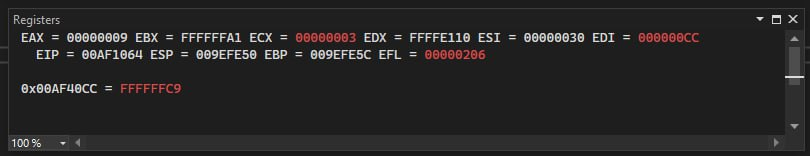
\includegraphics[width=0.90\textwidth]{iter2.jpg}
    \caption{Транспонування матриці}
\end{figure}

\paragraph{2.}Друга програма

\begin{verbatim}
.586p
.model flat, stdcall
_data segment
matrix   dd -17,   72,   11,   63,   36,   95
dd -36,  -99,   67,  -82,  -70,   39
dd -89,   48,   90,   75,   14,   -8
dd  86,   51,   37,   80,   59,   20
dd -68,   44,   -1,   84,   25,   45
dd -92,   62,   60,  -31,   78,   15
dd -56,  -20,  -69,  -49,  -58,   19
dd -65,  -38,  -30,   93,   10,   29
dd   9,  -85,  -95,  -55,   57,  -97

colCount equ 6
rowCount equ 9

transposedMatrix dd 6*9 dup(?) ; Transposed matrix


result DWORD ?            ; Result of dot product
sum9throw DWORD ?         ; Sum of the 9th row elements

_data ends
_text segment
start:
;mov ecx, 9 ; Number of rows
;mov ebx, 6 ; Number of columns

; Transpose the matrix
mov esi, 0 ; Row index
transpose_loop:
mov edi, 0 ; Column index
transpose_column_loop:
; Copy elements [matrix + esi*4*colCount + edi*4] to [transposedMatrix + edi*4 + esi*4]
imul ebx, esi, 4*colCount
imul edx, edi, 4*rowCount
mov eax, [matrix + ebx + edi*4]
mov [transposedMatrix + edx + esi*4], eax

inc edi
cmp edi, colCount
jl transpose_column_loop

inc esi
cmp esi, rowCount
jl transpose_loop

; Calculate the dot product of the first and third columns
mov edx, 0 ; Initialize dot product result to 0
mov edi, 0 ; Column index
mov esi, 0
dot_product_loop:
imul esi, edi, colCount
mov eax, [matrix + esi*4]          ; First column
mov ebx, [matrix + 2*4 + esi*4] ; Third column
imul eax, ebx
add edx, eax
inc edi
cmp edi, rowCount
jl dot_product_loop

; Calculate the sum of the 9th row elements that are >= -51 and <= 82
mov edi, 8*6*4 ; Start at the end of the 9th row
mov eax, 0     ; Initialize sum to 0
mov ecx, 6
sum_9th_row_loop:
cmp [matrix + edi], -51
jl skip_element
cmp [matrix + edi], 82
jg skip_element
add eax, [matrix + edi]
skip_element:
add edi, 4
loop sum_9th_row_loop

; Store the results
mov [result], edx      ; Dot product result
mov [sum9throw], eax   ; Sum of the 9th row elemen

ret
_text ends
end start

\end{verbatim}

\vspace{12pt}
\begin{figure}[H]
    \centering
    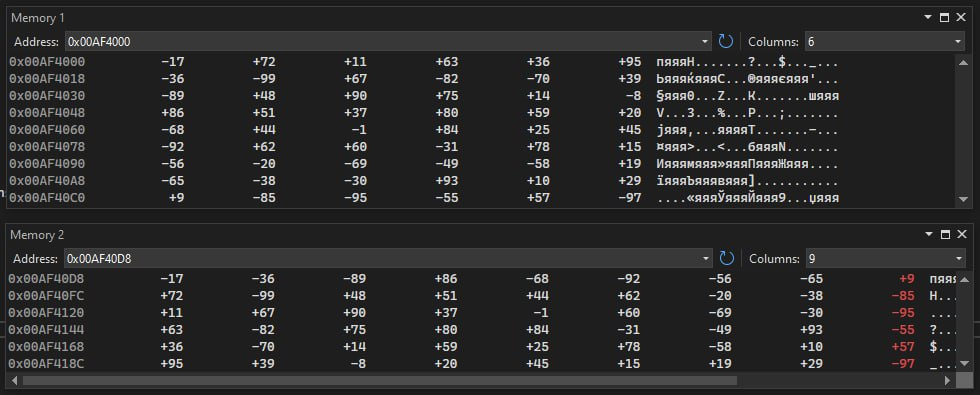
\includegraphics[width=0.90\textwidth]{matrix.png.jpg}
    \caption{Транспонування матриці}
\end{figure}
\begin{figure}[H]
    \centering
    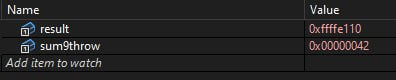
\includegraphics[width=0.90\textwidth]{matrix_vars.jpg}
    \caption{Змінні}
\end{figure}

\begin{figure}[H]
    \centering
    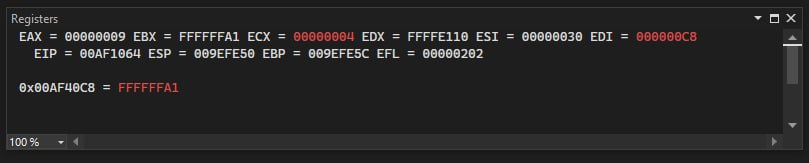
\includegraphics[width=0.90\textwidth]{iter1.jpg}
    \caption{Перша ітерація}
\end{figure}
\begin{figure}[H]
    \centering
    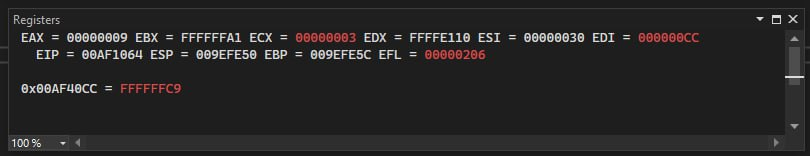
\includegraphics[width=0.90\textwidth]{iter2.jpg}
    \caption{Друга ітерація}
\end{figure}
\begin{figure}[H]
    \centering
    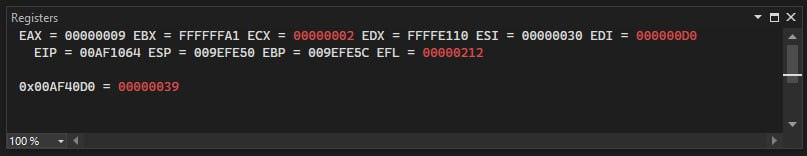
\includegraphics[width=0.90\textwidth]{iter3.jpg}
    \caption{Третя ітерація}
\end{figure}

\vspace{12pt}

\subsection*{Висновок} 
Я розібрався з базовим функціоналом асемблеру і як використовувати
Visual Studio для його відлагодження.


\end{document}